\chapter{Advanced Architectures}
In questo capitolo vengono presentate le architetture avanzate del cloud che vengono utilizzate per seguire i requisiti che il cloud si pone si soddisfare. La maggior parte di queste architetture riguardano il computing, e utilizzano i meccanismi di base visti nei capitoli precedenti. Le architetture avanzate rappresentano la formalizzazione dei domini funzionali, e definiscono le interazioni, i comportamenti e le combinazioni dei meccanismi e di altre componenti, e hanno come obiettivo offrire soluzioni specifiche.

\section{Hypervisor Clustering}
Quando vengono introdotti meccanismi per favorire la resilienza uno dei punti forti è dato dalla presenza dell'hypervisor. Essendo un punto critico, lo stesso hypervisor può essere soggetto a malfunzionamenti, per cui anche questa componente deve essere replicata e i meccanismi al suo interno devono essere gestiti. Questo è possibile grazie all'Hypervisor Clustering, che gestisce diversi server fisici assicurando il funzionamento delle varie macchine virtuali nonostante i malfunzionamenti che possono affliggere sia il server fisico che gli hypervisor. Quello che si fa normalmente nella migrazione di una macchina virtuale in casi di malfunzionamento viene fatto allo stesso modo per gli hypervisor: viene utilizzata una serie di hypervisor in esecuzione che possono prendere in carico diversi host. Il funzionamento è il seguente:
\begin{enumerate}
    \item I server fisici A, B e C rappresentano un cluster di server aventi lo stesso dominio di gestione, mentre gli hypervisor che sono eseguiti sui server hanno in carico un certo numero di macchine virtuali, la cui immagine si trova all'interno dello storage (3). Tutti gli hypervisor sono coordinati dalla VIM.
    \clearpage
    
    \begin{figure}[htb!]
    \centering
    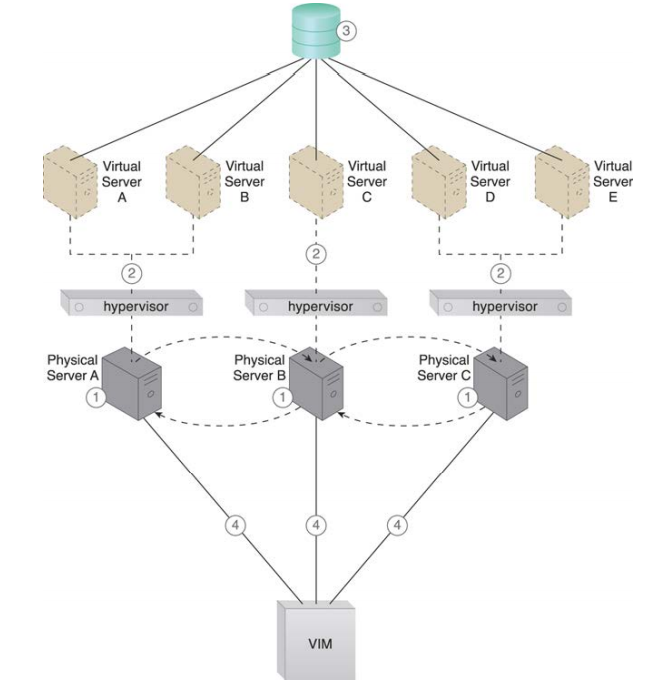
\includegraphics[width=9cm]{./Images/cap12/12.1.png}
    \end{figure}

    \item In ogni momento la comunicazione tra le macchine fisiche e la VIM avviene tramite messaggi di \textit{heartbeat}. Gli heartbeat sono tipi di messaggi che vengono scambiati a intervalli regolari tra i nodi del cluster. In caso di malfunzionamenti ci si rende subito conto quale nodo ha fallito perché non vengono inviati più messaggi di heartbeat.
    
    \begin{figure}[htb!]
    \centering
    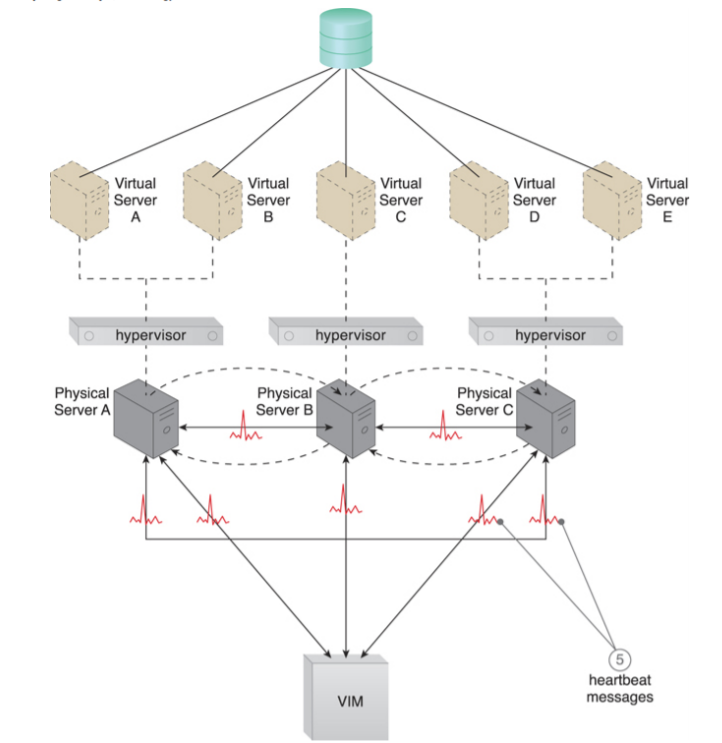
\includegraphics[width=9cm]{./Images/cap12/12.2.png}
    \end{figure}

    \item A questo punto si avvia un meccanismo di live migration grazie al quale le macchine virtuali si spostano dalla macchina fisica che ha fallito ad una funzionante passando per l'hypervisor. Questo è possibile grazie ai file immagine degli stati delle macchine che si trovano in uno storage condiviso. 
    
\end{enumerate}

I meccanismi utilizzati nell'Hypervisor Clustering sono:
\begin{itemize}
    \item Hypervisor
    \item Resource Cluster
    \item Logical Network Perimeter, in quanto tutte le componenti viste nel funzionamento devono risiedere nello stesso perimetro.
    \item Resource replication, attraverso il VIM agli hypervisor.
\end{itemize}

\section{Load Balanced Virtual Servers}
Un altro meccanismo avanzato del cloud è il bilanciamento del carico di lavoro, che serve per migliorare le prestazioni delle macchine e garantire un'alta qualità del servizio, come stabilito nei SLA. L'obiettivo quindi è quello di effettuare il bilanciamento del carico ma tra server fisici e non virtuali come il bilanciamento classico. Questo perché un server fisico potrebbe ricevere più carico di lavoro di quello che sopportare, anche a causa dei diversi server virtuali che sono in esecuzione su di esso. Quello che si fa allora è bilanciare il carico attraverso i server fisici per fare in modo che non siano sovraccaricati oppure sottoutilizzati. 

L'architettura del Load Balanced Virtual Server utilizza un \textit{capacity watchdog system} per calcolare le istanze di server virtuali e il loro carico di lavoro prima di distribuirlo al processing. Di seguito il funzionamento:
\begin{enumerate}
    \item L'architettura di Hypervisor Clustering fornisce le basi sulle quali è costruita l'architettura del Load Balanced Virtual Server (1). Le policy e le soglie di sopportamento sono definite nel watchdog capacity monitor (2), che confronta le capacità dei server fisici con il carico dei server virtuali in esecuziuoni su di essi (3). Invia quindi un segnale alla VIM indicando un sovraccarico (4).

    \begin{figure}[htb!]
    \centering
    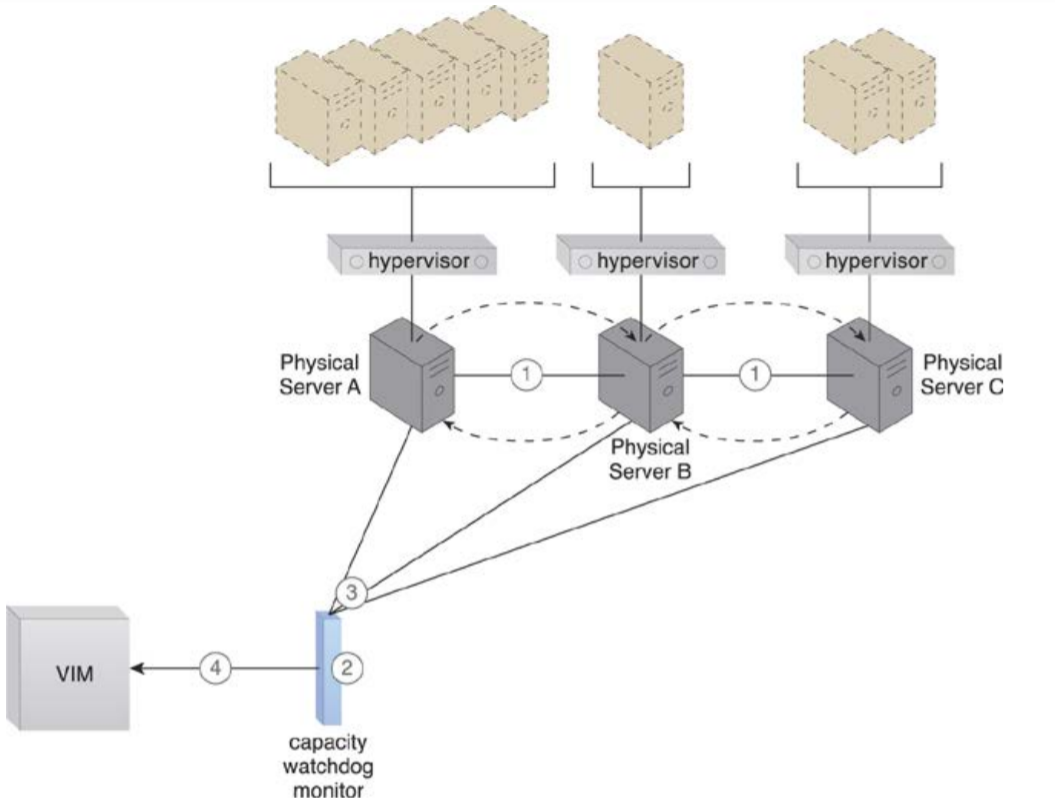
\includegraphics[width=9cm]{./Images/cap12/12.3.png}
    \end{figure}
    
    \item La VIM invia un segnale al load balancer per ridistribuire il carico basato sulle soglie predefinite (5). Il load balancer inizializza la Live Migration per spostare i virtual server (6), che quindi cambiano host.

    \begin{figure}[htb!]
    \centering
    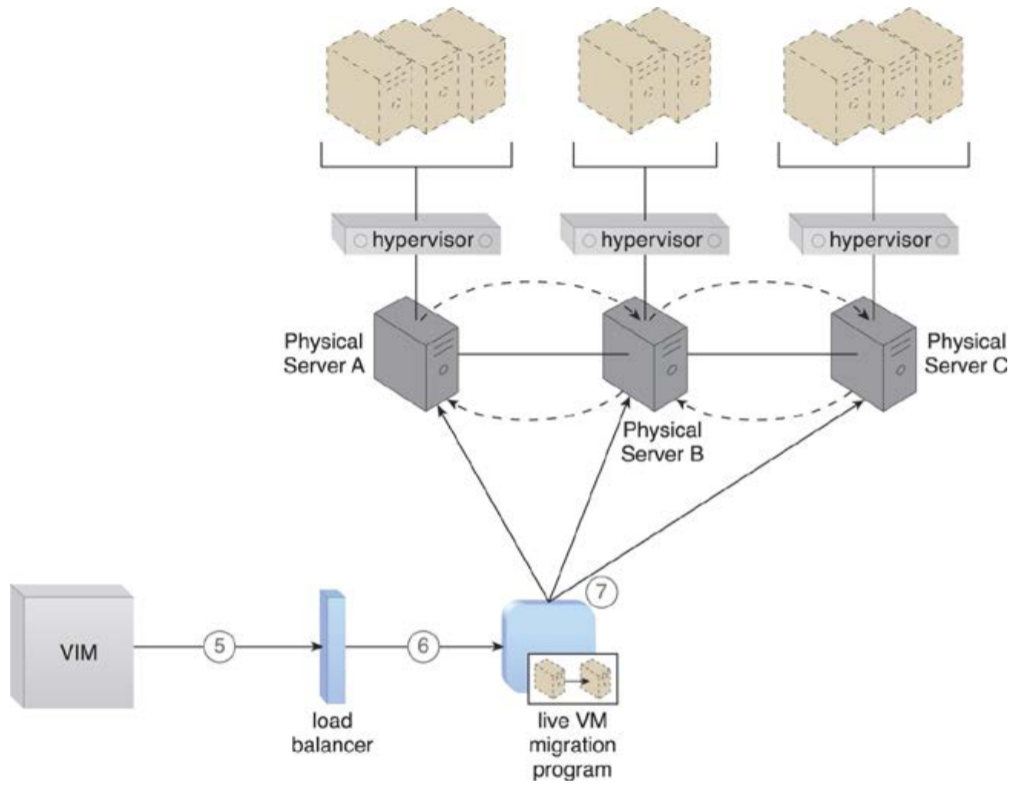
\includegraphics[width=9cm]{./Images/cap12/12.4.png}
    \end{figure}
    
    \item Il carico di lavoro viene bilanciato tra i server fisici presenti nel cluster. Il capacity watchdog monitor continua a monitorare il carico di lavoro e il consumo delle risorse (9).
    
    \begin{figure}[htb!]
    \centering
    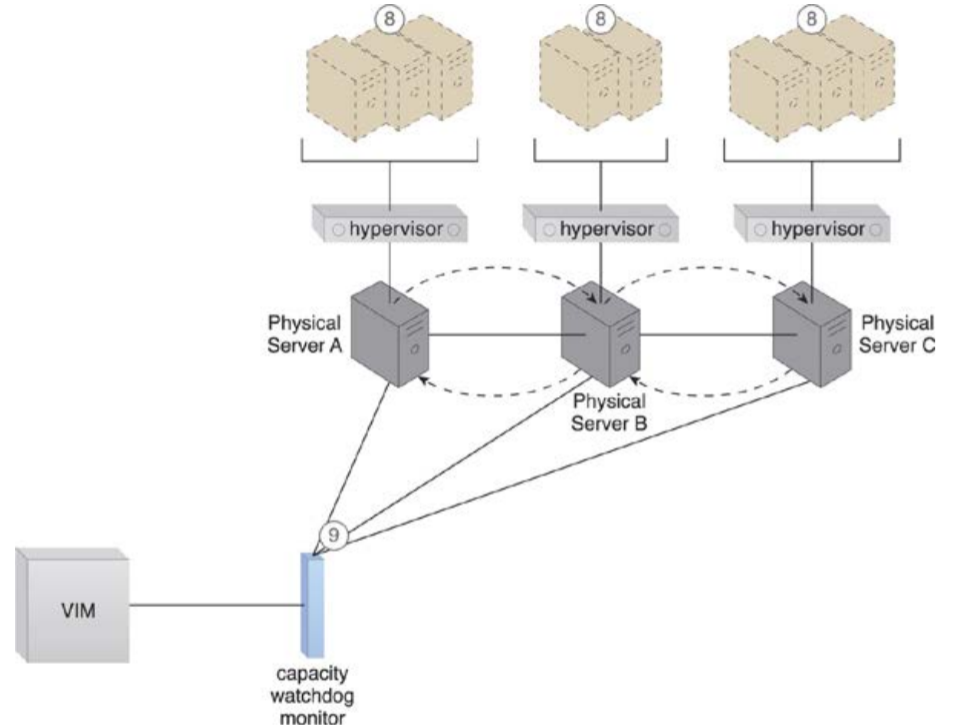
\includegraphics[width=9cm]{./Images/cap12/12.5.png}
    \end{figure}
    
\end{enumerate}

I meccanismi utilizzati sono:
\begin{itemize}
    \item Automated Scaling Listener
    \item Load Balancer
    \item Logical Network Perimeter
    \item Resource Replication
\end{itemize}
\clearpage

\section{Non-disruptive Service Relocation}
Mentre le architetture precedenti riguardavano principalmente il modello di deployment IaaS, quest'architettura e le successive riguardano più da vicino il modello SaaS: mentre prima andavano rilocati elementi della struttura, come server e hypervisor, qui vengono rilocati invece i servizi e le risorse non fisiche.

In base a ciò che viene definito nel SLA, i servizi devono essere sempre disponibili, e se un servizio non è disponibile le cause potrebbero essere diverse: numero di richieste troppo alto, aggiornamento o manutenzione del servizio. La rilocazione di un servizio viene realizzata attraverso il riconoscimento di un evento programmato e che suggerisce la duplicazione o la rimozione di un servizio a tempo di esecuzione - per questo si parla di non-disruptive relocation. Ciò può essere fatto in due modi:
\begin{itemize}
    \item il servizio viene temporaneamente spostato in un altro ambiente di hosting mentre è in esecuzione aggiungendo un'implementazione duplicata in un nuovo host;
    \item il servizio viene spostato permamentemente.
\end{itemize}
In ogni caso questa rilocazione deve assicurare la continuità del servizio: la nuova copia del servizio deve essere attiva e deve poter rispondere prima che la vecchia copia sia terminata.

Vediamo nel dettaglio il funzionamento:"
\begin{enumerate}
    \item L'Automated Scaling Listener monitora il carico di lavoro di un servizio cloud (1). La soglia predefinita del cloud service viene raggiunta quando il carico di lavoro aumenta (2), e ciò porta l'ASL ad inviare un messaggio alla VIM per iniziare la rilocazione (3). La VIM utilizza il meccanismo della Live VM Migration per fornire agli hypervisor coinvolti nella migrazione le informazioni necessarie per gestire una migrazione del servizio (4).
    
    \begin{figure}[htb!]
    \centering
    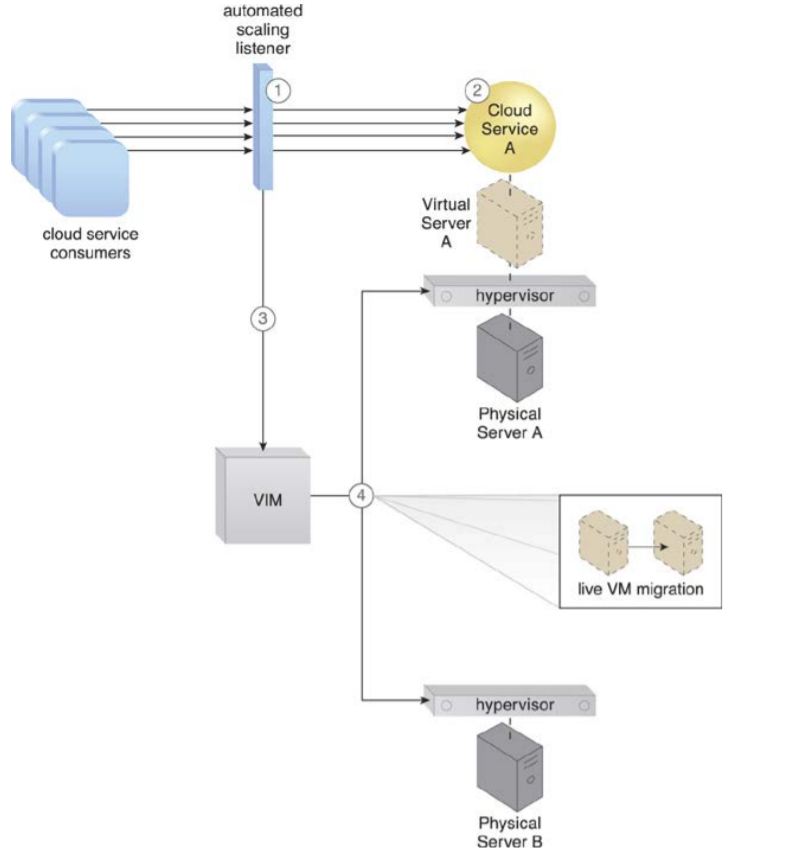
\includegraphics[width=9cm]{./Images/cap12/12.6.png}
    \end{figure}
    
    \item Una seconda copia del server virtuale e del servizio cloud sono creati dll'hypervisor di destinazione sul serevr fisico B (5).
    
    \begin{figure}[htb!]
    \centering
    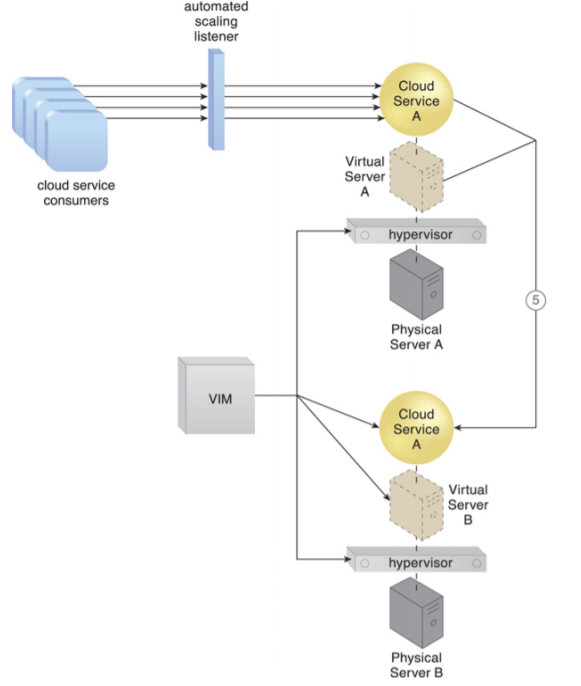
\includegraphics[width=7cm]{./Images/cap12/12.7.png}
    \end{figure}
    
    \item Lo stato di entrambi i server virtuali viene sincronizzato (6). L'istanza del primo virtual server viene rimossa dal server fisico A dopo che le richieste del cloud service consumer vengono reindirizzate correttamente verso la nuova istanza del servizio sul server fisico B (7). A questo punto le richieste del cloud service consumer vengono inviate permanentemente al server fisico B (8).
    
    \begin{figure}[htb!]
    \centering
    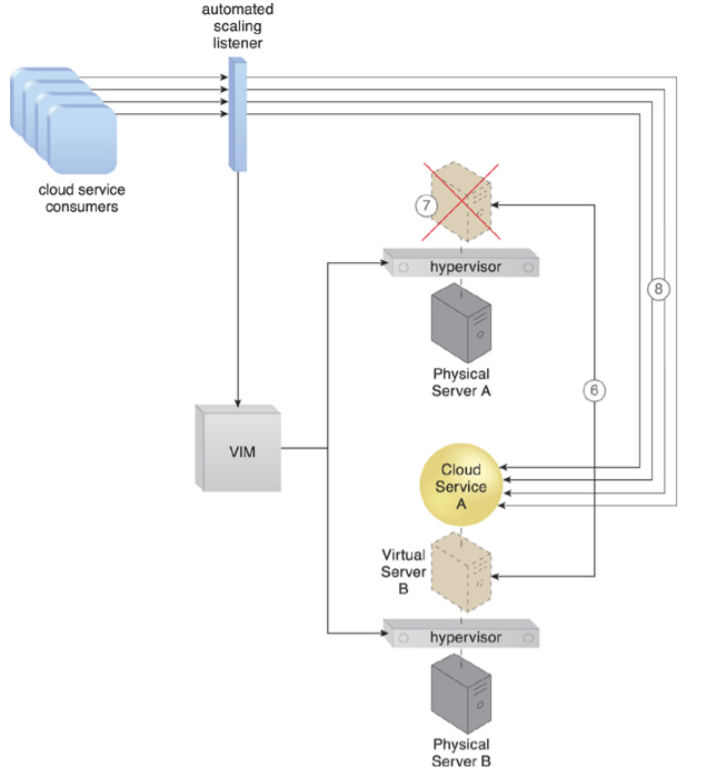
\includegraphics[width=7cm]{./Images/cap12/12.8.png}
    \end{figure}
    
\end{enumerate}

La \textbf{virtual server migration} è differente a seconda della locazione dei dischi e della configurazione del server. Inizialmente si fa una copia del disco sull'host di destinazione (in caso di storage remoto non condiviso oppure di storage locale). Dopo che la copia è stata creata, entrambe le istanze del server sono sincronizzate e i file sono rimossi dall'host originale. Se i file sono salvati su uno storage remoto condiviso, non è necessario copiare i file in quanto sono direttamente accessibili. A questo punto le autorizzazioni e i permessi del virtual server sono semplicemente trasferiti al nuovo server, e dunque lo stato viene automaticamente sincronizzato. In questo scenario acquistano importanza le configurazioni fissate di rete, in quanto anche cambiando host, questo si può connettere facilmente alla rete utilizzando le stesse impostazioni dell'host precedente.

I meccanismi utilizzati sono:
\begin{itemize}
    \item Automated Scaling Listener
    \item Load Balancer
    \item Cloud Storage Device
    \item Hypervisor
    \item Virtual Server
    \item Cloud Usage Monitor
    \item Pay-Per-Use Monitor, in quanto ogni volta che c'è una replicazione vengono calcolati i costi.
    \item Resource Replication
    \item SLA Management System
    \item SLA Monitor
\end{itemize}

\section{Zero Downtime}
Come sappiamo, un server fisico rappresenta un Single Point of Failure, quindi in caso di fallimento di un server potrebbe fallire l'intero sistema. Avere quindi la possibilità di offrire un sistema con zero downtime diventa difficile. La chiave di tutto questo meccanismo è un sistema di failover che permette ai server virtuali di essere spostati sui server fisici. L'idea anche qui si basa sul load balancing di file immagini di virtual server e di storage condiviso per poter fare la Live VM Migration. 

I meccanismi utilizzati sono:
\begin{itemize}
    \item Failover system
    \item Cloud Storage Device
    \item Virtual Server
    \item Audit Monitor, nel caso la rilocazione di un server abbia bisogno di una rilocazione dei dati. 
    \item Cloud Usage Monitor
    \item Hypervisor
    \item Logical Network Perimeter, in quanto ogni rilocazione viene fatta nello stesso perimetro.
    \item Resource Cluster
    \item Resource Replication, per gestire il pool di risorse che in questo caso sono le macchine virtuali.
\end{itemize}

\section{Cloud Balancing}
Mentre le architetture viste finora si basano su specifiche componenti, come sostituzione di hypervisor o di una singola risorsa, le prossime architetture riguardano una visione un po' più d'insieme. Ad esempio, quando le risorse vengono gestite da un load balancer attraverso diversi cloud, gli obiettivi sono:
\begin{itemize}
    \item migliorare le performance e la scalabilità delle risorse IT;
    \item aumentare la disponibilità e la reliability delle risorse IT;
    \item migliorare il bilanciamento del carico e l'ottimizzazione delle risorse IT. Non bisogna trascurare il fatto che diversi cloud possono avere diverse politiche di pricing e quindi \textit{ottimizzare} una risorsa può voler dire cose diverse in base al tipo di politica utilizzata.
\end{itemize}
Il meccanismo su scala più ampia è simile a quello già visto ma ovviamente con un numero maggiore di componenti dovuti alla maggiore dimensione. Il lavoro dell'Automated Scaling Listener è quello di redirigere le richieste del service consumer a una delle copie ridondanti di implementazione del servizio. Il sistema di failover si assicura che le risorse IT ridondanti siano capaci di gestire un failover cross-cloud, quindi che riguarda diversi provider. I malfunzionamenti sono annunciati, in modo che l'ASL possa evitare di inviare richieste alla risorsa che in quel momento non risponde o che è instabile. 

\begin{figure}[htb!]
    \centering
    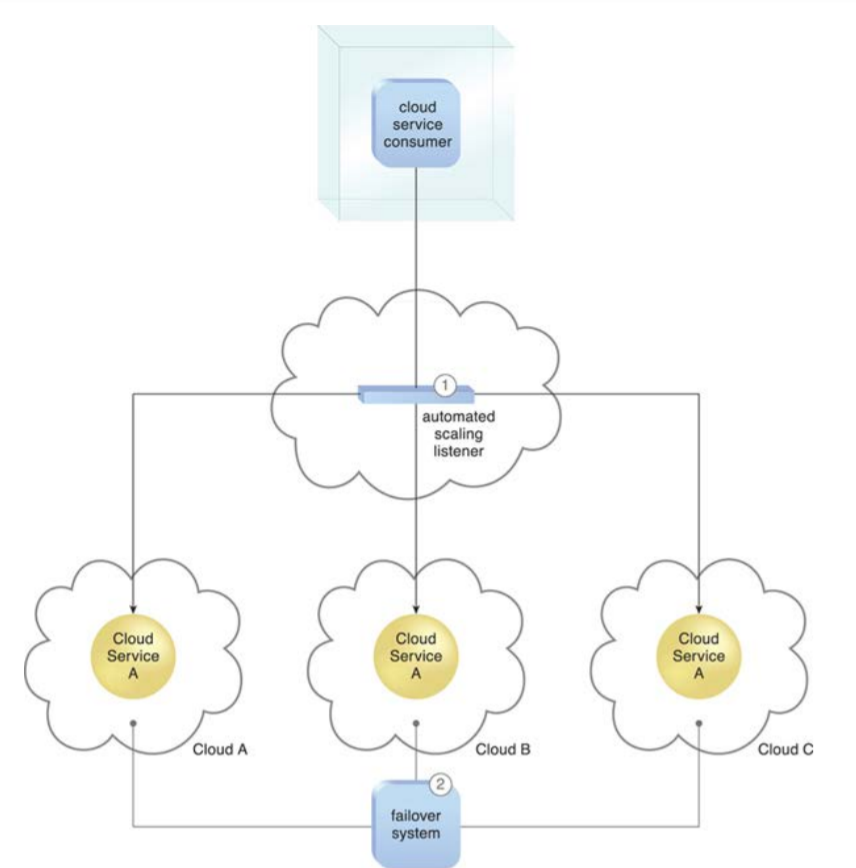
\includegraphics[width=9cm]{./Images/cap12/12.9.png}
\end{figure}

Nella figura possiamo vedere tre cloud provider che offrono lo stesso servizio. L'ASL è anch'esso su un cloud e il meccanismo di failover che è in grado di monitorare i vari provider permette di indirizzare le richieste dove decide l'Automated Scaling Listener. 

I meccanismi utilizzati sono:
\begin{itemize}
    \item Automated Scaling Listener
    \item Resource Replication
    \item Logical Network Perimeter
    \item Resource Replication (cross-cloud)
\end{itemize}

\section{Resource Reservation}
Un \textit{resource constraint} si ha quando a due o più consumer sono stati allocati una risorsa che non può essere condivisa oppure non ha abbastanza potenza. Un esempio è quando ci sono più macchine virtuali che si danneggiano l'una con l'altra, se stanno sulla stessa macchina fisica. Questo porta a un degrado delle prestazioni. Ci possono essere anche conflitti di prestiti non restituiti. La possibilità di potersi riservare una risorsa impatta sulla gestione delle risorse stesse: un customer può bloccare una serie di risorse mentre il resto del pool è ancora a disposizione per sharing e borrowing. Questo può essere fatto direttamente dal customer, e ovviamente ha un costo.

I meccanismi utilizzati sono:
\begin{itemize}
    \item Cloud Storage Device
    \item Virtual Server
    \item Audit Monitor: per controllare che le reservation siano in compliance con i permessi e le autorizzazioni del customer
    \item Cloud Usage Monitor
    \item Hypervisor
    \item Logical Network Perimeter
    \item Resource Replication
\end{itemize}

\section{Dynamic Failure Detect/Recovery}
I cloud sono composti da una grande quantità di risorse a cui accedono contemporaneamente moltissimi consumer. Queste risorse ovviamente possono fallire, quindi hanno bisogno di essere tenute sotto controllo. La gestione manuale delle risorse tipicamente non è la soluzione migliore da attuare in quanto inefficiente e poco pratica. Il meccanismo di Dynamic Failure Detect, che si basa sempre un watchdog, è in grado di rispondere automaticamente a una serie predefinita di scenari, come i failure. Notifica le failure condition se non possono essere risolte automaticameente. 
Un Cloud Usage Monitor più intelligente, che viene chiamato \textit{Intelligent Watchdog Monitor}, traccia le risorse IT e compie azioni predefinite in risposta ad eventi predefiniti, come ad esempio riavviare un servizio se questo non risponde, oppure riavviare l'intera macchina se questa dà problemi. Se nessun'azione va a buon fine, viene notificato l'admin.

\begin{figure}[htb!]
    \centering
    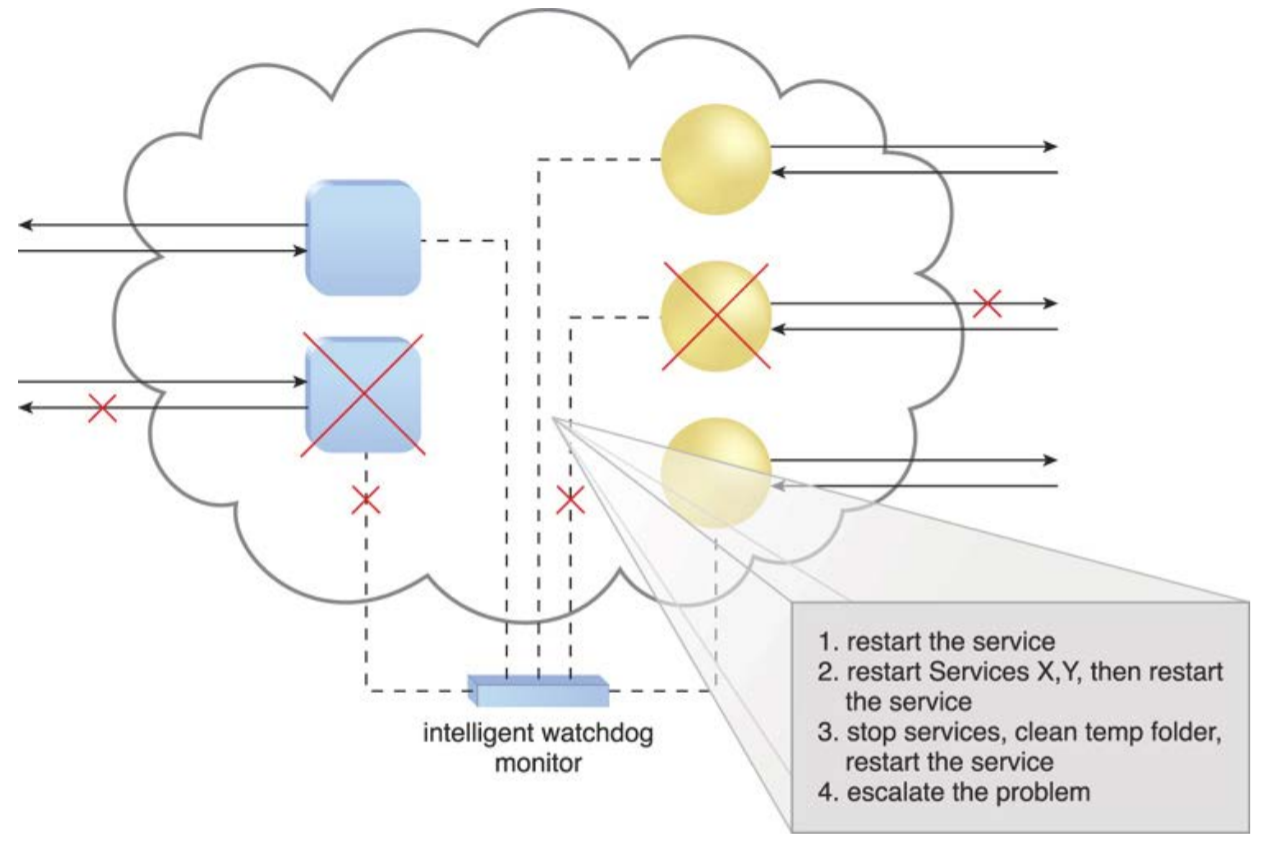
\includegraphics[width=9cm]{./Images/cap12/12.10.png}
\end{figure}

Tipicamente le azioni che vengono notificate sono:
\begin{itemize}
    \item esecuzione di file batch
    \item invio di un messaggio su terminale
    \item invio di un messaggio di testo
    \item invio di un messaggio email
    \item invio di una SNMP trap\footnote{\textit{Simple Network Management Protocol} (SNMP) è un protocollo di gestione di tutti gli apparati che stanno su un network. Una \textit{trap} è un metodo per indicare iun evento.}
    \item logging di un ticket
\end{itemize}

I meccanismi utilizzati sono:
\begin{itemize}
    \item Audit Monitor, per controllare che il recupero dei dati sia conforme alla legge e alle policy stabilite nei requisiti.
    \item Failover System
    \item SLA Management
\end{itemize}

\section{Bare-Metal Provisioning}
Normalmente il sistema remoto di management è nativo al sistema operativo dei vari server e quando il cloud provider deve fornire bare metal non può contare su questi sistemi di gestione remota: quindi il bare metal soffre della mancanza di gestione remota che permette a questi compiti di essere eseguiti con più facilita. Tipicamente queste opzioni si trovano nella ROM del server. L'architettura per attuare la fornitura di bare metal usa dei Service Agent specializzati che nel momento in cui il server parte, avvia il sistema di management remoto. Tipicamente a questi sistemi si accede via un'interfaccia web-based. 

Ovviamente ci sono delle attenzioni da pagare: una è la possibilità di errori, perché l'installazione è comunque eseguita da parte di una persona fisica, e l'altra è rappresentata dalle risorse necessarie offerte dal remote management software, che spesso richiedono risorse di calcolo molto potenti.

\vspace{5mm}

Le componenti dell'architettura sono:
\begin{itemize}
    \item \textbf{Discovery Agent}, che trova i server fisici liberi da assegnare ai cloud consumer.
    \item \textbf{Deployment Agent}, che viene installato nella memoria di un server fisico per fungere da client per la fornitura di bare metal.
    \item \textbf{Discovery Section}, che analizza la rete per trovare i server fisici a cui è possibile connettersi.
    \item \textbf{Management Loader}, che si connette al server fisico e carica le opzioni di gestione per il cloud consumer.
    \item \textbf{Deployment Component}, che server per installare il sistema operativo sui server fisici.
\end{itemize}
Questa infrastruttura software viene utilizzata per poter accedere a macchine fisiche e permettere al consumer di installare il sistema operativo richiesto su queste macchine.

Il bare metal provisioning viene fornito in maniera automatica: i consumer si collegano al software di gestione che già è preconfigurato per accogliere le richieste dei consumer, che possono configurare anche più macchine contemporaneamente o possono installare più sistemi operativi sulla stessa macchina. Il sistema di deployment centrale si connette ai server attraverso l'interfaccia di gestione e utilizza lo stesso protocollo per agire nella RAM della macchina fisica. A questo punto l'agente presente sulla macchina, senza ancora il sistema operativo, può configurarla per il SO che ha scelto il consumer.

I meccanismi utilizzati sono:
\begin{itemize}
    \item Cloud Storage Device, per salvare i template di sistemi operativi e i file di installazione
    \item Hypervisor
    \item Logical Network Perimeter, in quanto ai server fisici possono accedere sono i cloud consumer autorizzati.
    \item Resource Replication
    \item SLA Management System, perché il tipo di servizi che viene offerto può essere soggetto a restrizioni nel SLA.
\end{itemize}

\section{Rapid Provisioning}
Il processo di fornitura convenzionale può comprendere una serie di task che devono essere svolte manualmente. Nel cloud, la fornitura manuale di solito è inefficiente e soggetta ad errori, quindi non risulta adeguata. L'architettura del Rapid Provisioning automatizza la fornitura di una vasta famma di risorse IT, sia individualmente che in maniera colletiva.
Le componenti usate in quest'architettura comprendono un programma automatico di fornitura, un engine e degli script per poter gestire la fornitura di richieste on-demand. Inoltre ci sono componenti addizionali come server templates, application packages, custom scripts, sequence manager, sequence logger, operating system baseline, application configuration baseline e deployment data store. Ovviamente a seconda della risorsa si utilizza una combinazione di queste componenti.

\vspace{5mm}

Nel momento in cui l'utente utilizza il self-service portal per scegliere quali sono le caratteristiche, questo istruisce l'engine a rappresentare il cloud service che poi viene usato dall'amministratore della risorsa. Tutto il punto critico sta in queste due parti, che assicurano che tutto questo venga fatto automaticamente e senza interventi manuali di norma.

I meccanismi utilizzati sono:
\begin{itemize}
    \item Cloud Storage Device
    \item Resource Replication
\end{itemize}

\section{Storage Workload Management}
Il sovrautilizzo dei dispositivi di storage sul cloud aumenta ovviamente il carico di lavoro sullo storage controller, e causa problemi di prestazioni o spreco di risorse (nel caso di sottoutilizzo). Lo Storage Workload Management permette alle LUN di poter essere distribuite in maniera uniforme attraverso diversi dispositivi di cloud storage disponibili, come si può vedere nelle immagini successive.

I meccanismi utilizzati sono:
\begin{itemize}
    \item Audit Monitor
    \item Automated Scaling Listener
    \item Cloud Usage Monitor
    \item Load Balancer
    \item Logical Network Perimeter
\end{itemize}

\begin{figure}[htb!]
    \centering
    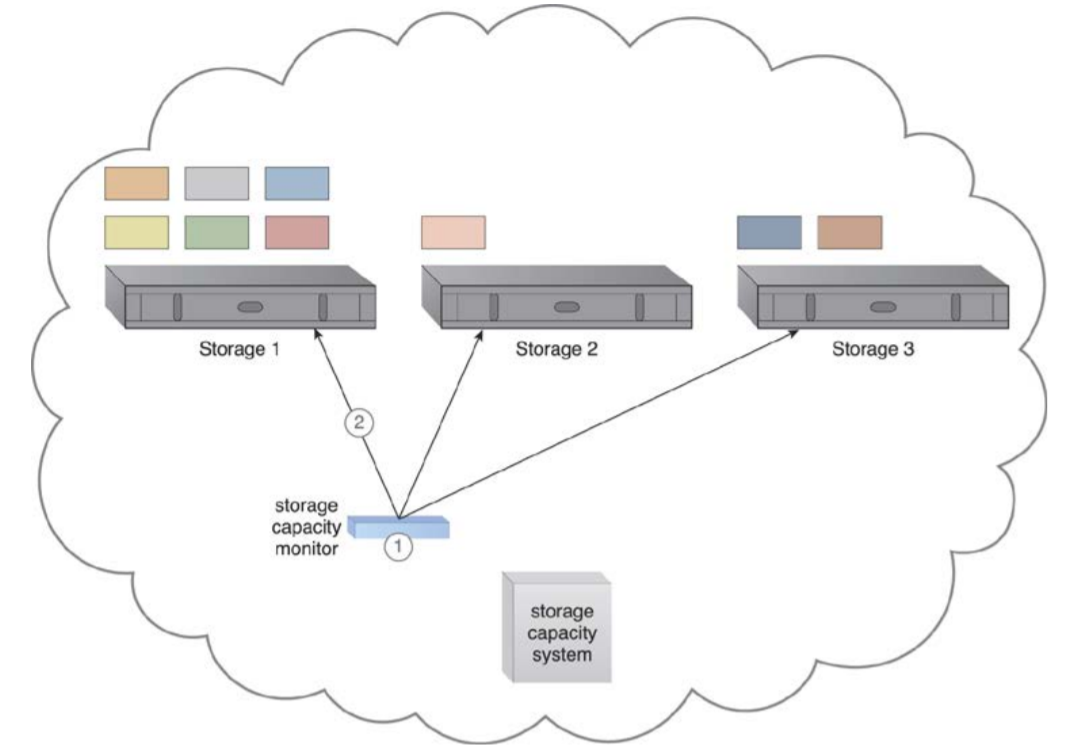
\includegraphics[width=9cm]{./Images/cap12/12.11.png}
\end{figure}

\begin{figure}[htb!]
    \centering
    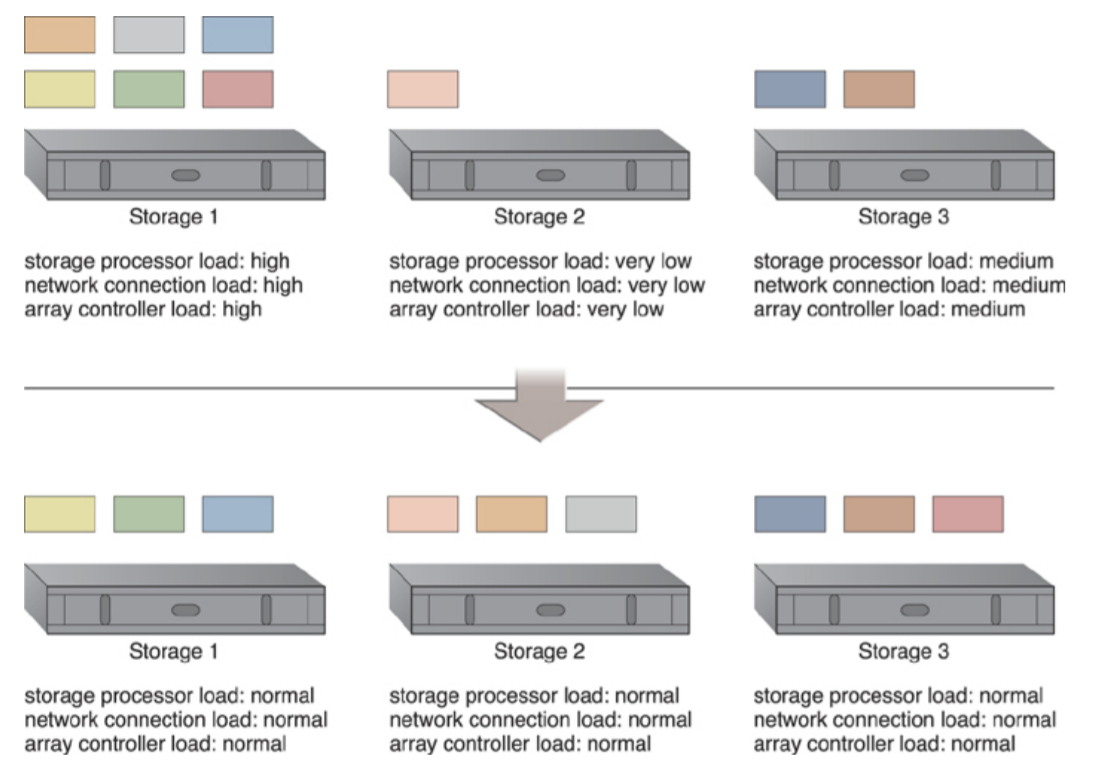
\includegraphics[width=9cm]{./Images/cap12/12.12.png}
\end{figure}

    \begin{figure}[htb!]
    \centering
    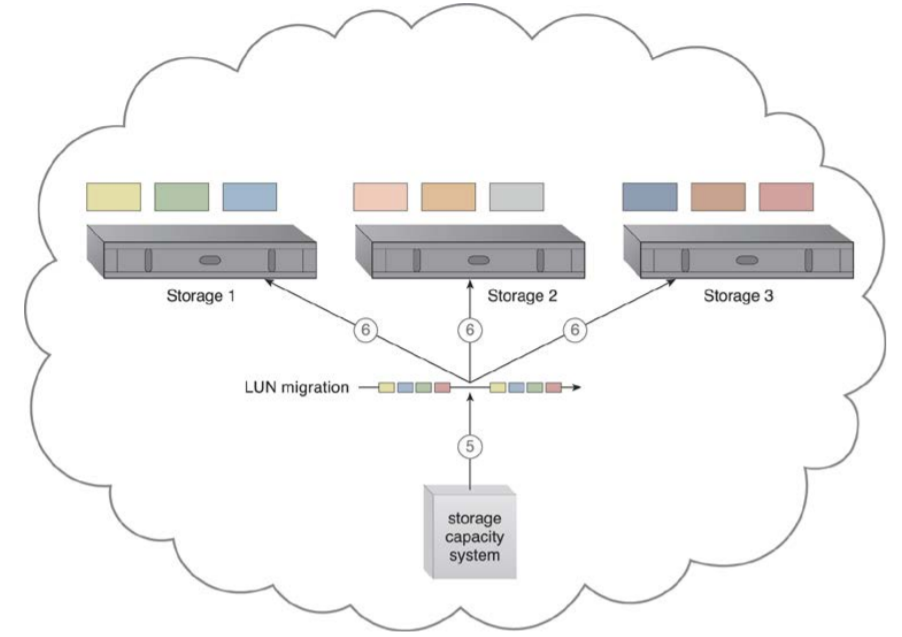
\includegraphics[width=9cm]{./Images/cap12/12.13.png}
\end{figure}

\clearpage
\section{Learning Check}
\begin{enumerate}
    \item Descrivi l'obiettivo dell'architettura Hypervisor Clustering e spiega come viene utilizzato l'hypervisor. Inoltre elenca i meccanismi del Cloud Computing utilizzati in questa architettura.
    \item Descrivi l'obiettivo dell'architettura Load Balanced Virtual Server Instances e spiega l'utilizzo delle policy di bilanciamento del carico e l'obiettico del Capacity Watchdog Monitor. Inoltre elenca i meccanismi del Cloud Computing utilizzati in questa architettura.
    \item Descrivi l'obiettivo dell'architettura Non-Disruptive Service Relocation e spiega come viene utilizzata la VIM e le sue componenti di live VM migration. Inoltre elenca i meccanismi del Cloud Computing utilizzati in questa architettura.
    \item Descrivi l'obiettivo dell'architettura Zero Downtime e spiega il suo utilizzo come sistema di resistenza ai fallimenti. Inoltre elenca i meccanismi del Cloud Computing utilizzati in questa architettura.
    \item Descrivi l'obiettivo dell'architettura Cloud Balancing e spiega come vengono utilizzati i meccanismi di Automated Scaling Listener e Resource Replication.
    \item Descrivi l'obiettivo dell'architettura Resource Reservation e descrivi a cosa serve il vincolo di condizione sulle risorse. Spiega anche come funziona lo scenario del prestito delle risorse. Inoltre elenca i meccanismi del Cloud Computing utilizzati in questa architettura.
    \item Descrivi l'obiettivo dell'architettura di Dynamic Failure Detection and Recovery e spiega come funziona il watchdog system e come si basa sul SLA monitor. Inoltre elenca i meccanismi del Cloud Computing utilizzati in questa architettura.
    \item Descrivi l'obiettivo dell'architettura Bare-Metal Provisioning e spiega l'utilizzo di un central deployment system e l'utilizzo di RAM visica via il meccanismo di remote management system. Inoltre elenca i meccanismi del Cloud Computing utilizzati in questa architettura.
    \item Descrivi l'obiettivo dell'architettura Rapid Provisioning ed elenca i meccanismi del Cloud Computing utilizzati in questa architettura.
    \item Descrivi l'obiettivo dell'architettura Storage Workload Management ed elenca i meccanismi del Cloud Computing utilizzati in questa architettura.
\end{enumerate}
